\documentclass[10pt,a4paper]{article}
\usepackage{amsmath,amssymb,amsthm,graphicx}
\usepackage{amsmath,amsfonts,amssymb,amsthm,graphicx}
\usepackage{hyperref}
\usepackage{thmtools,thm-restate}
\usepackage[capitalize,nameinlink]{cleveref}
\usepackage{tikz,enumerate}
\allowdisplaybreaks
\setcounter{MaxMatrixCols}{30}
\newtheorem{theorem}{Theorem}
\newtheorem{claim}[theorem]{Claim}
\newtheorem{corollary}[theorem]{Corollary}
\newtheorem{definition}[theorem]{Definition}
\newtheorem{lemma}[theorem]{Lemma}
\newtheorem{problem}[theorem]{Problem}
\newcommand{\<}{\langle}
\renewcommand{\>}{\rangle}
\DeclareMathOperator{\E}{\mathbb E}
\newcommand{\cl}[1]{\mathsf{#1}}
\newcommand{\ApxCount}{\mathsf{ApxCount}_{N,w}}
\newcommand{\AndApxCount}{\mathsf{AND}_2\circ\mathsf{ApxCount}_{N,w}}
\newcommand{\para}[1]{\paragraph{#1}}
\title{Approximate counting requires a large untrusted quantum witness or quadratically many membership queries}
\author{Scott Aaronson, Robin Kothari, William Kretschmer, Justin Thaler}
\date{doi:10.4230/LIPIcs.CCC.2020.7; CC BY 3.0 Unported}
\begin{document}
\maketitle
\noindent\textit{Editorial note.} Editable transcription of corresponding published CC BY3.0 Unported QMA problem/proof; nonexclusive nativev3 is private aid, not a public original. Selected public files exclude all unselected raw ranges/comments. FullSection2 andSection3 preserved, including original author constants/probability/parameter expressions without mathematical correction or added assumptions. Original restatable theorem numbers, equation offset and Figure3 restored; author TikZ figure retained as editable body with explicit actual package dependencies. Standard prior facts cited rather than recursively reproved. Native malformed optional bibliography label avoided by using formal published bibliographic text with original numbers. All production/validation solelyYupeng; root owns compilation.\par\medskip
\noindent\textit{Allowed standard prerequisites (editorial).}\begin{itemize}
\item Quantum query algorithms and QMA amplification; approximation theory and symmetric polynomial symmetrization. Full originalSection2 definitions/statements, source-local symmetrization proofs and guessing lemma retained; standard cited amplification is not recursively reproved
\end{itemize}\medskip
\section*{Approximate counting and the untrusted witness model}
\begin{problem}[Approximate Counting]
In the $\ApxCount$ problem, our goal is to decide whether a nonempty set $S\subseteq[N]$ satisfies $|S|\ge2w$ (YES) or $|S|\le w$ (NO), promised that one of these is the case.
\end{problem}
In the query model, the algorithm is given a membership oracle for $S$: one that, for any $i\in[N]$, returns whether $i\in S$.
In a QMA protocol, a skeptical verifier (Arthur) receives a quantum witness state $|\psi\rangle$ from an all-powerful but untrustworthy prover (Merlin), in support of the claim that $f(x)=1$. Arthur then needs to verify $|\psi\rangle$, via some algorithm that satisfies the twin properties of completeness and soundness. That is, if $f(x)=1$, then there must exist some $|\psi\rangle$ that causes Arthur to accept with high probability, while if $f(x)=0$, then every $|\psi\rangle$ must cause Arthur to reject with high probability. We call such a protocol a QMA protocol for computing $f$.

\begin{restatable}{theorem}{qmabound}
\label{thm:qmabound}
Consider a $\mathsf{QMA}$ protocol that solves $\ApxCount$. If the protocol receives a quantum witness of length $m$, and makes $T$ queries to the membership oracle for $S$, then
either $m = \Omega(w)$ or 
$ T = \Omega\bigl(\sqrt{N/w}\bigr)$.
\end{restatable}

This lower bound proved in \Cref{sec:QMA} resolves the $\mathsf{QMA}$ complexity of  $\ApxCount$, as (up to a $\log N$ factor) it matches the cost of two trivial $\mathsf{QMA}$ protocols.
In the first, Merlin sends $2w$ items claimed to be in $S$,
and Arthur picks a constant number of the items at random
and confirms they are all in $S$ with one membership query each. 
This protocol has witness length $m=O(w\log N)$ (the number of bits needed to specify $2w$ elements out of $N$) and $T=O(1)$. 
In the second protocol, Merlin does nothing, and Arthur solves the problem with $T=O\bigl(\sqrt{N/w}\bigr)$ quantum queries.

\begin{restatable}{theorem}{sbqp}
\label{thm:sbqp}
Consider an $\mathsf{SBQP}$ algorithm for $\AndApxCount$ that makes $T$ queries to membership oracles for the two instances of $\ApxCount$. Then $T=\Omega\left(\min\bigl\{w,\sqrt{N/w}\bigr\}\right)$.
\end{restatable}

\setcounter{section}{1}
\setcounter{theorem}{5}
\setcounter{equation}{4}
\setcounter{figure}{2}
\section{Preliminaries}

\label{sec:prelim}

In this section we introduce some definitions and known facts about
polynomials and complexity classes.

%
\subsection{Approximation theory}
\label{s:approxprelim}
We will use several results from approximation theory,\ each of which has
previously been used (in some form) in other applications of the polynomial
method to quantum lower bounds. \ We start with the basic inequality of A.A.
Markov \cite{markov1890question}.

\begin{lemma}[Markov]
\label{markovlem}Let $p$\ be a real polynomial, and suppose that
\begin{equation}
\max_{x,y\in\left[ a,b\right] }\left\vert p\left( x\right) -p\left( y\right)
\right\vert \leq H.
\end{equation}
Then for all $x\in\left[ a,b\right] $, we have
\begin{equation}
\left\vert p^{\prime}\left( x\right) \right\vert \leq\frac{H}{b-a}\deg\left(
p\right) ^{2},
\end{equation}
where $p^{\prime}(x)$ is the derivative of $p$ at $x$.
\end{lemma}

We'll also need a bound that was explicitly stated by Paturi \cite{paturi},
and which amounts to the fact that, among all degree-$d$
polynomials that are bounded within a given range, the Chebyshev polynomials
have the fastest growth outside that range.

\begin{lemma}[Paturi]
\label{paturilem}Let $p$\ be a real polynomial, and suppose that $\left\vert
p\left( x\right) \right\vert \leq1$\ for all $\left\vert x\right\vert \leq1$
. \ Then for all $x\leq1+\mu$, we have
\begin{equation}
\left\vert p\left( x\right) \right\vert \leq\exp\left( 2\deg\left( p\right)
\sqrt{2\mu+\mu^{2}}\right) .
\end{equation}
\end{lemma}

We now state a useful corollary of \Cref{paturilem}, which says (in effect)
that slightly shrinking the domain of a low-degree real polynomial can only
modestly shrink its range.

\begin{corollary}
\label{paturicor}Let $p$\ be a real polynomial of degree $d$, and suppose
that
\begin{equation}
\max_{x,y\in\left[ a,b\right] }\left\vert p\left( x\right) -p\left( y\right)
\right\vert \geq H.
\end{equation}
Let $\varepsilon\leq\frac{1}{100d^{2}}$\ and $a^{\prime}:=a+\varepsilon
\left( b-a\right) $. \ Then
\begin{equation}
\max_{x,y\in\left[ a^{\prime},b\right] }\left\vert p\left( x\right) -p\left(
y\right) \right\vert \geq\frac{H}{2}.
\end{equation}
\end{corollary}

\begin{proof}
Suppose by contradiction that
\begin{equation}
\left\vert p\left(  x\right)  -p\left(  y\right)  \right\vert <\frac{H}{2}
\end{equation}
for all $x,y\in\left[  a^{\prime},b\right]  $. \ By affine shifts, we can
assume without loss of generality that $\left\vert p\left(  x\right)
\right\vert <\frac{H}{4}$\ for all $x\in\left[  a^{\prime},b\right]  $. \ Then
by \Cref{paturilem}, for all $x\in\left[  a,b\right]  $\ we have
\begin{equation}
\left\vert p\left(  x\right)  \right\vert <\frac{H}{4}\cdot\exp\left(
2d\sqrt{2\left(  \frac{1}{1-\varepsilon}-1\right)  +\left(  \frac
{1}{1-\varepsilon}-1\right)  ^{2}}\right)  \leq\frac{H}{2}.
\end{equation}
But this violates the hypothesis.
\end{proof}

We will also need a bound that relates the range of a low-degree polynomial
on a discrete set of points to its range on a continuous interval. \ The
following lemma generalizes a result due to Ehlich and Zeller \cite{ez} and
Rivlin and Cheney \cite{rc}, who were interested only in the case where the
discrete points are evenly spaced.

\begin{lemma}
\label{ezrclem}Let $p$\ be a real polynomial of degree at most $\sqrt{k}$,
and let $0=z_{1}<\cdots<z_{M}=k$\ be a list of points such that $
z_{i+1}-z_{i}\leq1$\ for all $i$ (the simplest example being the integers $
0,\ldots,k$). \ Suppose that
\begin{equation}
\max_{x,y\in\left[ 0,k\right] }\left\vert p\left( x\right) -p\left( y\right)
\right\vert \geq H.
\end{equation}
Then
\begin{equation}
\max_{i,j}\left\vert p\left( z_{i}\right) -p\left( z_{j}\right) \right\vert
\geq\frac{H}{2}.
\end{equation}
\end{lemma}

\begin{proof}
Suppose by contradiction that
\begin{equation}
\left\vert p\left(  z_{i}\right)  -p\left(  z_{j}\right)  \right\vert
<\frac{H}{2}
\end{equation}
for all $i,j$. \ By affine shifts, we can assume without loss of generality
that $\left\vert p\left(  z_{i}\right)  \right\vert <\frac{H}{4}$\ for all
$i$. \ Let
\begin{equation}
c:=\max_{x\in\left[  0,k\right]  }\frac{\left\vert p\left(  x\right)
\right\vert }{H/4}.
\end{equation}
If $c\leq1$, then the hypothesis clearly fails, so assume $c>1$. \ Suppose
that the maximum, $\left\vert p\left(  x\right)  \right\vert =\frac{cH}{4}$,
is achieved between $z_{i}$\ and $z_{i+1}$. \ Then by basic calculus, there
exists an $x^{\ast}\in\left[  z_{i},z_{i+1}\right]  $\ such that
\begin{equation}
\left\vert p^{\prime}\left(  x^{\ast}\right)  \right\vert >\frac{2\left(
c-1\right)  }{z_{i+1}-z_{i}}\cdot\frac{H}{4}\geq\frac{\left(  c-1\right)
H}{2}.
\end{equation}
So by \Cref{markovlem},
\begin{equation}
\frac{\left(  c-1\right)  H}{2}<\frac{cH/4}{k}\deg\left(  p\right)  ^{2}.
\end{equation}
Solving for $c$, we find
\begin{equation}
c<\frac{2k}{2k-\deg\left(  p\right)  ^{2}}\leq2.
\end{equation}
But if $c<2$, then $\max_{x\in\left[  0,k\right]  }\left\vert p\left(
x\right)  \right\vert <\frac{H}{2}$, which violates the hypothesis.
\end{proof}

We also use a related inequality due to Coppersmith and Rivlin~\cite
{coppersmith-rivlin} that bounds a polynomial on a continuous interval in
terms of a bound on a discrete set of points, but now with the weaker
assumption that the degree is at most $k$, rather than $\sqrt{k}$. \ This
gives a substantially weaker bound.

\begin{lemma}[Coppersmith and Rivlin]
\label{lem:coppersmith_rivlin} Let $p$ be a real polynomial of degree at
most $k$, and suppose that $\left\vert p(x)\right\vert \leq 1$ for all
integers $x\in \{0,1,\ldots ,k\}$. \ Then there exist universal constants $
a,b$ such that for all $x\in \lbrack 0,k]$, we have
\begin{equation}
\left\vert p(x)\right\vert \leq a\cdot \exp \left( b\,\deg (p)^{2}/k\right) .
\end{equation}
\end{lemma}


%
\subsection{Symmetric polynomials}

\para{Univariate symmetrizations.}
Our starting point is the well-known \textit{symmetrization lemma} of Minsky
and Papert \cite{mp} (see also Beals et al.\ \cite{bbcmw}\ for its
application to quantum query complexity), by which we can often reduce
questions about multivariate polynomials to questions about univariate ones.

\begin{lemma}[Minsky--Papert symmetrization]
\label{symlem} Let $p:\left\{ 0,1\right\} ^{N}\rightarrow\mathbb{R}$\ be a
real multilinear polynomial of degree $d$, and let $q:\{0,1,\ldots,N\}\to
\mathbb{R}$ be defined as
\begin{equation}
q\left( k\right) :=\E_{\left\vert X\right\vert =k}\left[ p\left( X\right) 
\right] .
\end{equation}
Then $q$ can be written as a real polynomial in $k$ of degree at most $d$.
\end{lemma}

We now introduce a different, lesser known
notion of symmetrization, 
which we call the \emph{erase-all-subscripts} symmetrization
for reasons to be explained shortly. This symmetrization previously appeared in \cite{shi} under the name ``linearization,'' and it is also equivalent to the noise operator used in analysis of Boolean functions \cite[Definition 2.46]{odonnell}.

\begin{lemma}[Erase-all-subscripts
symmetrization]
Let $p:\left\{ 0,1\right\} ^{N}\rightarrow\mathbb{R}$\ be a
real multilinear polynomial of degree $d$,
and for
any real number $k \in [0, 1]$,
let $M_{k}$ denote
the distribution over $\{0, 1\}^N$, wherein each coordinate is selected
independently to be 1 with probability $k$.
Let $q:[0, 1] \to
\mathbb{R}$ be defined as
\begin{equation}
q\left( k\right) :=\E_{X \sim M_{k}}\left[ p\left( X\right) 
\right] .
\end{equation}
Then $q$ can be written as a real polynomial in $k$ of degree at most $d$.
\label{lem:eraseallsubscripts}
\end{lemma}
\begin{proof} (see, for example, \cite[Proof of Theorem 3]{STT12}).
Given the multivariate polynomial expansion of $p$,
we can obtain $q$ easily just by ``erasing all the subscripts in each variable''. For example, if
$p(x_1, x_2, x_3)= 2 x_1 x_2 + x_2 x_3 + x_2$, we replace every $x_i$ with $k$ to obtain
$q(k)=2k\cdot k+ k\cdot k + k=3k^2 + k$.
This follows from linearity of expectation along with the fact that $M_k$
is defined to be the
product distribution wherein
each coordinate has expected value $k$.
\end{proof}

We highlight the following key difference between Minsky--Papert symmetrization
and the erase-all-subscripts symmetrization. Let $p:\left\{ 0,1\right\} ^{N}\rightarrow [0, 1]$
be a real multivariate polynomial whose evaluations at Boolean inputs are in
$[0, 1]$, i.e., for all $x\in\{0,1\}^n$, we have $p(x)\in[0,1]$.
If $q$ is the erase-all-subscripts symmetrization of $p$, 
then $q$ takes values in $[0,1]$ at all \emph{real-valued}
inputs in $[0, 1]$: $q(k) \in [0,1]$ for all $k \in [0,1]$. 
If $q$ is the Minsky--Papert symmetrization of $p$,
then it is only guaranteed to take values in $[0,1]$ at 
\emph{integer-valued} inputs in $[0, N]$, i.e., $q(k)\in [0,1]$ 
is only guaranteed to hold at $k\in\{0,1,\ldots,N\}$.
This is the main reason we use erase-all-subscripts symmetrization
in this work.

\para{Bivariate symmetrizations.}
In this paper, it will be convenient
to consider bivariate versions of both
Minsky--Papert and erase-all-subscripts
symmetrization, and their applications to oracle separations. To this end,
define $X\in \left\{ 0,1\right\} ^{N}$, the \textquotedblleft characteristic
string\textquotedblright\ of the set $S\subseteq \left[ N\right] $, by $
x_{i}=1$\ if $i\in S$\ and $x_{i}=0$\ otherwise. \ Let $\mathcal{O}_{S}$
denote the unitary that performs a membership query to $S$, defined as
\begin{equation}
\mathcal{O}_{S}\left\vert i\right\rangle \left\vert b\right\rangle
=(1-2bx_{i})\left\vert i\right\rangle \left\vert b\right\rangle
\end{equation}
for any index $i\in \lbrack N]$ and bit $b\in \{0,1\}$.

Because we study oracle intersection problems, it is often convenient to
think of an algorithm as having access to \textit{two} oracles, wherein the
first bit in the oracle register selects the choice of oracle. \ As a
consequence, we need a slight generalization of a now well-established fact
in quantum complexity: that the acceptance probability of a quantum
algorithm with an oracle can be expressed as a polynomial in the bits of the
oracle string.

\begin{lemma}[Symmetrization with two oracles]
\label{lem:symmetrization} Let $Q^{\mathcal{O}_{S_{0}},\mathcal{O}_{S_{1}}}$
be a quantum algorithm that makes $T$ queries to a pair of membership
oracles for sets $S_{0},S_{1}\subseteq \lbrack N]$. \ Let $D_{\mu }$ denote
the distribution over subsets of $[N]$ wherein each element is selected
independently with probability $\frac{\mu }{N}$. \ Then there exist
bivariate real polynomials $q(s,t)$ and $p(x,y)$ of degree at most $2T$
satisfying:
\begin{align*}
\textrm{for all real numbers } s, t \in [0, N],& \quad
q(s,t)=\E_{\substack{ S_{0}\sim D_{s}, \\ S_{1}\sim D_{t}}}\left[ \Pr [Q^{
\mathcal{O}_{S_{0}},\mathcal{O}_{S_{1}}}\text{ accepts}]\right], \textrm{ and} \\
\textrm{for all integers } x, y \in \{0, 1, \dots, N\},& \quad
p(x,y)=\E_{\substack{ |S_{0}|=x, \\ |S_{1}|=y}}\left[ \Pr [Q^{\mathcal{O}
_{S_{0}},\mathcal{O}_{S_{1}}}\text{ accepts}]\right].
\end{align*}
\end{lemma}

\begin{proof}
Take $X = X_0|X_1$ to be the concatenation of the characteristic strings of the two oracles, and let $S \subseteq [2N]$ be such that $X$ is the characteristic string of $S$. Then, Lemma 4.2 of Beals et al.\ \cite{bbcmw} tells us that there is a real multilinear polynomial $r(X)$ of degree at most $2T$ in the bits of $X$ such that $r(X) = \Pr[ Q^{\mathcal{O}_S} \text{ accepts}]$.

Observe that $r$ has a meaningful probabilistic interpretation over arbitrary inputs in $[0, 1]$. A vector $X \in [0, 1]^{2N}$ of probabilities corresponds to a distribution over $\{0,1\}^{2N}$ wherein each bit is chosen from a Bernoulli distribution with the corresponding probability. Because $r$ is multilinear, $r$ in fact computes the expectation of the acceptance probability over this distribution. In particular, the polynomial
\begin{equation}
q(s, t) = r\bigg(\underbrace{\frac{s}{N},\ldots,\frac{s}{N}}_{N \text{ times}}, \underbrace{\frac{t}{N},\ldots,\frac{t}{N}}_{N \text{ times}}\bigg) = \E_{\substack{S_0 \sim D_s,\\S_1 \sim D_t}}\left[\Pr[ Q^{\mathcal{O}_{S_0},\mathcal{O}_{S_1}} \text{ accepts}] \right]    
\end{equation}
corresponds to selecting $S_0 \sim D_s$ and $S_1 \sim D_t$. The total degree of $q$ is obviously
at most the degree of $r$, by the same reasoning as in the proof of \Cref{lem:eraseallsubscripts}.

To construct $p$, we apply the symmetrization lemma of Minsky and Papert \cite{mp} to symmetrize $r$, first with respect to $X_0$, then with respect to $X_1$:
\begin{equation}
    p_0(x, X_1) = \E_{|S_0|=x} r(X_0,X_1) =  \E_{|S_0|=x}\left[\Pr[ Q^{\mathcal{O}_{S_0},\mathcal{O}_{S_1}} \text{ accepts}] \right]
\end{equation}
\begin{equation}
    p(x, y) = \E_{|S_1|=y} p_0(x,X_1) = \E_{\substack{|S_0|=x,\\|S_1|=y}}\left[\Pr[ Q^{\mathcal{O}_{S_0},\mathcal{O}_{S_1}} \text{ accepts}] \right] 
\end{equation}  
The degree of $p$ is at most the degree of $r$, due to \Cref{symlem}.
\end{proof}


We remark that, as a consequence of their definitions in \Cref{lem:symmetrization}, $p$ and $q$ satisfy:
\begin{equation}
q(s, t) = \E \left[ p(X, Y) \right],
\end{equation}
where $X$ and $Y$ are drawn from $N$-trial binomial distributions with means $s$ and $t$, respectively.

\para{Symmetric Laurent polynomials.}
Finally, we state a useful fact about Laurent polynomials:

\begin{lemma}[Symmetric Laurent polynomials]
\label{lem:symmetric} Let $\ell (x)$ be a real Laurent polynomial of positive
and negative degree $d$ that satisfies $\ell (x)=\ell (1/x)$. \ Then there exists a (ordinary) real
polynomial $q$ of degree $d$ such that $\ell (x)=q(x+1/x)$.
\end{lemma}

\begin{proof}
$\ell(x) = \ell(1/x)$ implies that the coefficients of the $x^i$ and $x^{-i}$ terms are equal for all $i$, as otherwise $\ell(x) - \ell(1/x)$ would not equal the zero polynomial. Thus, we may write $\ell(x) = \sum_{i=0}^d a_i \cdot (x^i + x^{-i})$ for some coefficients $a_i$. So, it suffices to show that $x^i + x^{-i}$ can be expressed as a polynomial in $x + 1/x$ for all $0 \le i \le d$.

We prove by induction on $i$. The case $i = 0$ corresponds to constant polynomials. For $i > 0$, by the binomial theorem, observe that $(x + 1/x)^i = x^i + x^{-i} + r(x)$ where $r$ is a degree $i - 1$ real Laurent polynomial satisfying $r(x) = r(1/x)$. By the induction assumption, $r$ can be expressed as a polynomial in $x + 1/x$, so we have $x^i + x^{-i} = (x + 1/x)^i - r(x)$ is expressed as a polynomial in $x + 1/x$.
\end{proof}

%
\subsection{Complexity classes}

\begin{definition}
\label{def:qma}
The complexity class $\mathsf{QMA}$ consists of the
languages $L$ for which there exists a quantum polynomial time
verifier $V$ with the following properties:

\begin{enumerate}
\item Completeness: if $x \in L$, then there exists a quantum witness state $|\psi\>$ on $\mathrm{poly}(|x|)$ qubits such that $\Pr\left[V(x, |\psi\>) \text{ accepts}\right] \ge \frac{2}{3}$.

\item Soundness: if $x \not\in L$, then for any quantum witness state $|\psi\>$ on $\mathrm{poly}(|x|)$ qubits, $\Pr\left[V(x, |\psi\>) \text{ accepts}\right] \le \frac{1}{3}$.
\end{enumerate}
\end{definition}

A quantum verifier that satisfies the above
promise for a particular language will be referred to as a $\mathsf{QMA}$
verifier or $\mathsf{QMA}$ protocol throughout.

Though $\mathsf{SBP}$ and $\mathsf{SBQP}$ can be defined in terms of
counting complexity functions, for our purposes it is easier to
work with the following equivalent definitions (see B\"ohler et al.\ \cite
{BGM06}):

\begin{definition}
\label{def:sbp_sbqp} The complexity class $\mathsf{SBP}$ consists of the
languages $L$ for which there exists a probabilistic polynomial time
algorithm $M$ and a polynomial $\sigma$ with the following properties:

\begin{enumerate}
\item If $x \in L$, then $\Pr\left[M(x) \text{ accepts}\right] \ge
2^{-\sigma(|x|)}$.

\item If $x \not\in L$, then $\Pr\left[M(x) \text{ accepts}\right] \le
2^{-\sigma(|x|)}/2$.
\end{enumerate}

The complexity class $\mathsf{SBQP}$ is defined analogously, wherein the
classical algorithm is replaced with a quantum algorithm.
\end{definition}

A classical (respectively, quantum) algorithm that satisfies the above
promise for a particular language will be referred to as an $\mathsf{SBP}$
(respectively, $\mathsf{SBQP}$) algorithm throughout. \ Using these
definitions, a  query complexity relation between $\mathsf{QMA}$
protocols and $\mathsf{SBQP}$ algorithms follows from the procedure of
Marriott and Watrous \cite{marriott}, which shows that one can exponentially
improve the soundness and completeness errors of a $\mathsf{QMA}$ protocol
without increasing the witness size. \ 
This relationship is now standard; see
for example \cite[Remark 6]{marriott} or \cite[Proposition 4.2]
{sherstov2019vanishing} for a proof of the following lemma:

\begin{lemma} 
\label{lem:guessing} Suppose there is a $\mathsf{QMA}$ protocol for some
problem that makes $T$ queries and receives an $m$-qubit witness. \ Then
there is a quantum query algorithm $Q$ for the same problem that makes $O(mT)$ queries, and satisfies the following:

\begin{enumerate}
\item If $x \in L$, then $\Pr\left[Q(x) \text{ accepts}\right] \ge
2^{-m}$.

\item If $x \not\in L$, then $\Pr\left[Q(x) \text{ accepts}\right] \le
2^{-10m}$.
\end{enumerate}
\end{lemma}


%

\section{QMA complexity of approximate counting}

\label{sec:SBPQMA}

This section establishes
an 
optimal lower bound on the $\mathsf{QMA}$
complexity of approximate counting.
We first lower bound the $\mathsf{SBQP}$ complexity
of the $\mathsf{AND}_2 \circ \mathsf{ApxCount}_{N,w}$ problem (
\Cref{thm:sbqp}). 
This implies a $\mathsf{QMA}$ lower bound
for $\mathsf{ApxCount}_{N,w}$ via \Cref{lem:guessing},
but it is not quantitatively optimal. 
We prove the optimal $\mathsf{QMA}$ lower bound 
(\Cref{thm:qmabound}) via
\Cref{lem:betterforqma}, which
leverages additional properties 
of 
the $\mathsf{SBQP}$ protocol derived via
\Cref{lem:guessing}
from any $\mathsf{QMA}$ protocol with small
witness length. Finally, \Cref{cor:qma_separation}
describes new oracle separations that
are immediate consequences of \Cref{thm:qmabound} and \Cref{thm:sbqp}. 

%
\subsection{Lower bound for \texorpdfstring{$\mathsf{SBQP}$}{SBQP} algorithms}
\label{sec:SBQP} 

Our lower bound on the $\cl{SBQP}$ complexity of $\AndApxCount$ hinges 
on the following theorem. \ The theorem
uses Laurent polynomials to prove a degree lower bound for bivariate
polynomials that satisfy an upper bound on an \textquotedblleft
L\textquotedblright -shaped pair of rectangles and a lower bound at a nearby
point:

\begin{theorem}
\label{thm:L} Let $0<w<32w<N$ and $M\geq 1$. \ Let $R_{1}=[4w,N]\times \lbrack 0,w/2]$ and
$R_{2}=[0,w/2]\times \lbrack 4w,N]$ be disjoint rectangles in the plane, and
let $L=R_{1}\cup R_{2}$. \ Let $p(x,y)$ be a real polynomial of degree $d$
with the following properties:
\begin{enumerate}
\item $p(4w, 4w) \ge 1.5 \cdot M$.
\item $0 \le p(x, y) \le 1$ for all $(x, y) \in L$.
\end{enumerate}
Then $d = \Omega(\sqrt{N/w} \cdot \log M)$.
\end{theorem}

\begin{figure}[tbp]
\centering
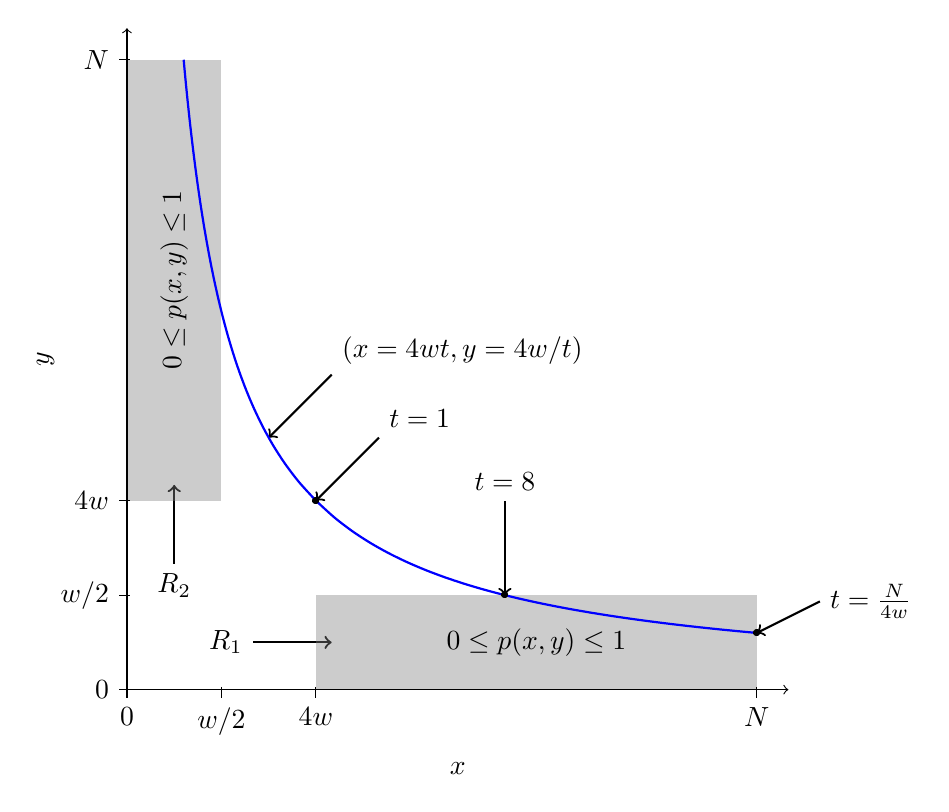
\begin{tikzpicture}[y=0.4cm, x=0.4cm]
	\pgfmathsetmacro{\N}{20}
	\pgfmathsetmacro{\w}{3}
	\pgfmathsetmacro{\tw}{\w+\w}
	\pgfmathsetmacro{\Np}{\N+1}

%
	\draw[<-,thick] (\tw+0.5, \w/2) -- (\w+1,\w/2) node[anchor=east] {$R_1$};
	\draw[<-,thick] (\w/2, \tw+0.5) -- (\w/2,\w+1) node[anchor=north] {$R_2$};

%
	\fill[gray,opacity=.4] (\tw,0) -- (\tw,\w) -- (\N,\w) -- (\N,0);
	\fill[gray,opacity=.4] (0,\tw) -- (\w,\tw) -- (\w,\N) -- (0,\N);

%
	\draw[->] (0,0) -- coordinate (x axis mid) (\Np,0);
    	\draw[->] (0,0) -- coordinate (y axis mid) (0,\Np);
    	
%
	\draw[<-,thick] (\tw,\tw) -- (\tw+2,\tw+2) node[anchor=south west] {$t=1$};   	
	\draw[<-,thick] (\w*4,\w) -- (\w*4,\w*2) node[anchor=south] {$t=8$};
	\draw[<-,thick] (\N,4*\w*\w/\N) -- (\N+2,1+4*\w*\w/\N) node[anchor=west] {$t=\frac{N}{4w}$};
	\draw[<-,thick] (1.5*\w,2*\w*4/3) -- (1.5*\w+2,2*\w*4/3+2) node[anchor=south west] {$(x=4wt,y=4w/t)$};
    	
    \draw (0,1pt) -- (0,-3pt) node[anchor=north] {0};
    \draw (\w,1pt) -- (\w,-3pt) node[anchor=north] {$w/2$\vphantom{l}};
    \draw (\tw,1pt) -- (\tw,-3pt) node[anchor=north] {$4w$};
    \draw (\N,1pt) -- (\N,-3pt) node[anchor=north] {$N$};

    \draw (1pt,0) -- (-3pt,0) node[anchor=east] {0};
    \draw (1pt,\w) -- (-3pt,\w) node[anchor=east] {$w/2$};
    \draw (1pt,\tw) -- (-3pt,\tw) node[anchor=east] {$4w$};
    \draw (1pt,\N) -- (-3pt,\N) node[anchor=east] {$N$};

%
	\node[below=0.8cm] at (x axis mid) {$x$};
	\node[rotate=90, above=0.8cm] at (y axis mid) {$y$};
	\node at (\w+\N/2, \w/2) {$0 \le p(x, y) \le 1$};
	\node[rotate=90] at (\w/2, \w+\N/2) {$0 \le p(x, y) \le 1$};

     \draw[thick,domain=1:{\N/(2*\w)},smooth,variable=\t,blue] plot ({2*\w*\t},{2*\w/\t});
%
     \draw[thick,domain=1:{\N/(2*\w)},smooth,variable=\t,blue] plot ({2*\w/\t},{2*\w*\t});
     \node at ({\w+\w},{\w+\w}) {\tiny\textbullet};
     \node at (4*\w,\w) {\tiny\textbullet};
     \node at (\N,4*\w*\w/\N) {\tiny\textbullet};
\end{tikzpicture}
\caption{Diagram of \Cref{thm:L} (not drawn to scale).}
\label{fig:L}
\end{figure}

\begin{proof}
Observe that if $p(x, y)$ satisfies the statement of the theorem, then so does $p(y, x)$. This is because the constraints in the statement of the theorem are symmetric in $x$ and $y$ (in particular, because $R_1$ and $R_2$ are mirror images of one another along the line $x = y$; see \Cref{fig:L}). As a result, we may assume without loss of generality that $p$ is symmetric, i.e.,\ $p(x, y) = p(y, x)$. Else, we may replace $p$ by $\frac{p(x, y) + p(y, x)}{2}$ because the set of polynomials that satisfy the inequalities in the statement of the theorem are closed under convex combinations.

Consider the hyperbolic parametric curve $(x = 4wt, y=4w/t)$ as it passes through $R_1$ (see \Cref{fig:L}). We can view the restriction of $p(x, y)$ to this curve as a Laurent polynomial $\ell(t) = p(4wt, 4w/t)$ of positive and negative degree $d$. The bound of $p(x,y)$ on all of $R_1$ implies that $|\ell(t)| \le 1$ when $t \in [8, \frac{N}{4w}]$ and that $\ell(1) \ge 1.5$ (see \Cref{fig:L}). Moreover, the condition that $p(x, y)$ is symmetric implies that $\ell(t) = \ell(1/t)$.

By \Cref{lem:symmetric} for symmetric Laurent polynomials, $\ell(t)$ can be viewed as a degree $d$ polynomial $q(t + 1/t)$. Under the transformation $s = t + 1/t$, $q$ satisfies $|q(s)| \le 1$ for $s \in [8 + 1/8, \frac{N}{4w} + \frac{4w}{N}]$ and $q(2) \ge 1.5 M$. Note that the length of the interval $[8 + 1/8, \frac{N}{4w} + \frac{4w}{N}]$ is $\Theta(N/w)$ because $w < N$. By an appropriate affine transformation of $q$, we can conclude from \Cref{paturilem} with $\mu = \Theta(w/N)$ that $d = \Omega(\sqrt{N/w} \cdot \log M)$.
\end{proof}

Why is \Cref{thm:L} useful? \ One may be tempted to apply this theorem
directly to the polynomial $p(x,y)$ obtained in \Cref{lem:symmetrization} to
conclude a degree lower bound (and thus a query complexity lower bound), as
the \textquotedblleft L\textquotedblright -shaped pair of rectangles $
L=R_{1}\cup R_{2}$ correspond to \textquotedblleft no\textquotedblright\
instances of $\mathsf{AND}_{2}\circ \mathsf{ApxCount}_{N,w}$, while $(4w,4w)$
corresponds to a \textquotedblleft yes\textquotedblright\ instance. \
However, even though $p(x,y)$ is bounded at lattice points in $L$, it need
not be bounded along the entirety of $L$.\footnote{
One can nevertheless use this intuition to obtain a nontrivial (though
suboptimal) lower bound by inspecting $p$ alone. Using the Markov brothers'
inequality (\Cref{markovlem}), if $\deg (p)=o(\sqrt{w})$, then the bounds on
$p(x,y)$ at lattice points in $L$ imply that $|p(x,y)|\leq 1+o_{w}(1)$ for
all $(x,y)\in L$. Thus, \Cref{thm:L} applies if $\deg (p)=o(\sqrt{w})$, so
overall we get a lower bound of $\Omega \left( \min \left\{ \sqrt{w},\sqrt{
N/w}\right\} \right) $ for the $\mathsf{SBQP}$ query complexity of $\mathsf{
AND}_{2}\circ \mathsf{ApxCount}_{N,w}$. See 
\href{https://arxiv.org/abs/1902.02398}{arXiv:1902.02398} for details.} \ 

To obtain a lower bound, we
instead use the connection between the polynomials $p(x,y)$ and $q(s,t)$
from \Cref{lem:symmetrization}, and establish \Cref{thm:sbqp} from the
introduction, restated for convenience:

\sbqp*

\begin{proof}
Let $N > 32w$ (otherwise the theorem holds trivially). Since $Q$ is an $\mathsf{SBQP}$ algorithm, we may suppose that $Q$ accepts with probability at least $2\alpha$ on a ``yes'' instance and with probability at most $\alpha$ on a ``no'' instance (note that $\alpha$ may be exponentially small in $N$). Take $p(x,y)$ and $q(s, t)$ to be the symmetrized bivariate polynomials of degree at most $2T$ defined in \Cref{lem:symmetrization}. Define $L' = ([0, w] \times [0, w]) \cup ([0, w] \times [2w, N]) \cup ([2w, N] \times [0, w])$. The conditions on the acceptance probability of $Q$ for all $S_0, S_1$ that satisfy the $\ApxCount$ promise imply that $p(x, y)$ satisfies these corresponding conditions:
\begin{enumerate}
\item $1 \ge p(x, y) \ge 2\alpha$ for all $(x, y) \in \left([2w, N] \times [2w, N]\right) \cap \mathbb{Z}^2$.
\item $0 \le p(x, y) \le \alpha$ for all $(x, y) \in L' \cap \mathbb{Z}^2$.
\end{enumerate}

Our strategy is to show that if $T = o(w)$, then these conditions on $p$ imply that the polynomial $q(s, t) \cdot \frac{0.9}{\alpha}$ satisfies the statement of \Cref{thm:L} for all sufficiently large $w$. This in turn implies $T = \Omega(\sqrt{N/w})$. This allows us conclude that either $T = \Omega(w)$ or $T = \Omega(\sqrt{N/w})$, which proves the theorem.

Suppose $T = o(w)$, so that $p(x, y)$ and $q(s, t)$ both have degree $d=o(w)$. We begin by upper bounding $p(x, y)$ at the lattice points $(x, y)$ outside of $L'$. 
We claim the following:
\begin{enumerate}[(a)]
\item $|p(x, y)| \le \alpha \cdot a \cdot \exp(bd^2 / w) \le \alpha \cdot a \cdot \exp(bd)$ whenever $(x, y) \in L'$ and either $x$ or $y$ is an integer, where $a$
and $b$ are the constants from \Cref{lem:coppersmith_rivlin}. This follows from \Cref{lem:coppersmith_rivlin} by fixing either $x$ or $y$ to be an integer and viewing the resulting restriction of $p(x, y)$ as a univariate polynomial in the other variable.
\item $|p(x, y)| \le \alpha \cdot a \cdot \exp(bd) \cdot \exp(2\sqrt{3}d) = \alpha \cdot a \cdot \exp((b + 2\sqrt{3})d)$ whenever $x \in [w, 2w]$, $y \in [0, w]$, and $y$ is an integer. This follows \Cref{paturilem}: consider the univariate polynomial $p(\cdot, y)$ on the intervals $[0, w]$ and $[2w, 3w]$, where it is bounded by (a).
\item $|p(x, y)| \le \alpha \cdot a \cdot \exp((b + 2\sqrt{3})d) \cdot a \cdot \exp(bd^2/w) \le \alpha \cdot a^2 \cdot \exp((2b + 2\sqrt{3})d)$ whenever $x \in [w, 2w]$ and $y \in [0, w]$. This follows from \Cref{lem:coppersmith_rivlin}: consider the univariate polynomial $p(x, \cdot)$ on the interval $[0, w]$, where it is bounded at integer points by (b).
\item $|p(x, y)| \le \alpha \cdot a^2 \cdot \exp((2b + 2\sqrt{3})d) \cdot \exp(4dy/w) = \alpha \cdot a^2 \cdot \exp((2b + 2\sqrt{3} + 4y/w)d)$ whenever $x \in [0, N]$, $y \in [w + 1, N]$, and $x$ is an integer. This follows from  \Cref{paturilem}: consider the univariate polynomial $p(x, \cdot)$ on the interval $[0, w]$, where it is bounded by (a) when $x \in [0, w]$ or $x \in [2w, N]$, or bounded by (c) when $x \in [w, 2w]$. 
By an affine shift, this corresponds to applying \Cref{paturilem} with $\mu = 2y/w - 2$, with the observation that $\sqrt{2\mu + \mu^2} < \mu + 2$.
\end{enumerate}

We now use this to upper bound $q(s, t)$ when $s \in [4w, N]$ and $t \in [0, w/2]$. Let $X$ and $Y$ be drawn from $N$-trial binomial distributions with means $s$ and $t$, respectively,
so that $q(s, t) = \E[p(X,Y)]$. Using the above bounds and basic probability, we have 
\begin{align}
0 \leq q(s, t) = \E[p(X,Y)] &\le \alpha \cdot \bigg( \Pr[X \ge 2w, Y \le w] + \Pr[X \le 2w, Y \le w] \cdot a \cdot \exp\left(\left(b+2\sqrt{3}\right)d\right)  \nonumber \\
& \quad + \sum_{y = w+1}^N \Pr[Y = y] \cdot a^2 \cdot \exp\left(\left(2b + 2\sqrt{3} + 4y/w\right)d\right) \bigg)\\
&\le \alpha \cdot \bigg(1 + \Pr[X \le 2w] \cdot a \cdot \exp\left(\left(b+2\sqrt{3}\right)d\right)   \nonumber \\
& \quad + \sum_{y = w+1}^N \Pr[Y \ge y] \cdot a^2 \cdot \exp\left(\left(2b + 2\sqrt{3} + 4y/w\right)d\right)\bigg).
\end{align}
The probabilities above are easily bounded with a Chernoff bound:
\begin{align}
q(s, t)=\E[p(X,Y)] &\le \alpha \cdot \bigg( 1 + a \cdot \exp\left(\left(b+2\sqrt{3}\right)d - w/2\right)  \nonumber\\
& \quad + \sum_{y = w+1}^N a^2 \cdot \exp\left(\left(2b + 2\sqrt{3} + 4y/w\right)d - y/6\right)\bigg).
\end{align}
Because $a$ and $b$ are universal constants from \Cref{lem:coppersmith_rivlin}, when $d = o(w)$, the first exponential term becomes arbitrarily small for all sufficiently large $w$. Moreover, for all sufficiently large $w$, the remaining sum becomes bounded by a geometric sum. For some constant $c$, we have
\begin{align*}
\sum_{y = w+1}^N a^2 \cdot \exp\left(\left(2b + 2\sqrt{3} + 4y/w\right)d - y/6\right) &\le \sum_{y = w+1}^\infty c \cdot \exp\left(-y/12\right)\\
&\le \frac{c}{1 - \exp(-1/12)} \cdot \exp(-w/12)\\
&= o_w(1).
\end{align*}
Thus we conclude that $0 \le q(s, t) \le \alpha \cdot (1 + o_w(1))$ when $s \in [4w, N]$ and $t \in [0, w/2]$ (i.e.,\ $(s, t) \in R_1$ in the statement of \Cref{thm:L}). By symmetry, we can conclude the same bound when $s \in [0, w/2]$ and $t \in [4w, N]$ (i.e.,\ $(s, t) \in R_2$ in the statement of \Cref{thm:L}).

Now, we lower bound $q(4w, 4w)$. Let $X$ and $Y$ be drawn from independent $N$-trial binomial distributions with mean $4w$, so that $q(4w, 4w) = \mathbb{E}\left[p(X,Y)\right]$. Then we have 
\begin{align*}
\mathbb{E}\left[p(X,Y)\right] &\ge 2\alpha \cdot \Pr[X \ge 2w, Y \ge 2w]\\
&\ge 2\alpha \cdot \left(1 - \Pr[X \le 2w] - \Pr[Y \le 2w]\right)\\
&\ge 2\alpha \cdot \left(1 - 2\exp(-w/2)\right)\\
&\ge 2\alpha \cdot (1 - o_w(1))
\end{align*}
We conclude that $q(s, t) \cdot \frac{0.9}{\alpha}$ satisfies the statement of \Cref{thm:L} (with $M=1$) for all sufficiently large $w$.
\end{proof}

We remark that this lower bound is tight, i.e.,\ there exists an $\mathsf{
SBQP}$ algorithm that makes $O\left( \min \left\{ w,\sqrt{N/w}\right\}
\right) $ queries. \ The $O(\sqrt{N/w})$ upper bound follows from the $
\mathsf{BQP}$ algorithm of Brassard, H{\o }yer, and Tapp \cite{bht:count}. \
The $O(w)$ upper bound is in fact an $\mathsf{SBP}$ upper bound with the
following algorithmic interpretation: first, guess $w+1$ items randomly from
each of $S_{0}$ and $S_{1}$. \ Then, verify using the membership oracle that
the first $w+1$ items all belong to $S_{0}$ and that the latter $w+1$ items
all belong to $S_{1}$, accepting if and only if this is the case. \ Clearly,
this accepts with nonzero probability if and only if $\left\vert
S_{0}\right\vert \geq w+1$ and $\left\vert S_{1}\right\vert \geq w+1$. 

%
\subsection{Lower bound for \texorpdfstring{$\mathsf{QMA}$}{QMA}}
\label{sec:QMA} 

In this section, we establish the optimal $\mathsf{QMA}$ lower bound 
(\Cref{thm:qmabound}).
We begin by quantitatively improving the $\mathsf{SBQP}$
lower bound for $\AndApxCount$ of \Cref{thm:sbqp},
under the stronger assumption that the parameter $\alpha$ 
in the $\mathsf{SBQP}$ protocol is not smaller than $2^{-w}$.
(In addition to a stronger
conclusion, this assumption also permits a considerably simpler
analysis than was required to prove \Cref{thm:sbqp}).

\begin{lemma}
\label{lem:betterforqma}
Consider any quantum query algorithm $Q^{\mathcal{O}_{S_{0}},\mathcal{O}_{S_{1}}}$
for $\AndApxCount$
that makes $T$ queries to the membership oracles
$\mathcal{O}_{S_{0}}$ and $\mathcal{O}_{S_{1}}$
for the two instances of $\ApxCount$ and
satisfies the following. For some $m=o(w)$, $\alpha=2^{-m}$, and $M \in [1, \alpha^{-1}]$:
\begin{enumerate}
\item If $x \in L$, then $\Pr\left[Q(x) \text{ accepts}\right] \ge
\alpha$.
\item If $x \not\in L$, then $\Pr\left[Q(x) \text{ accepts}\right] \le
\alpha/(2 M)$.
\end{enumerate}
Then $T = \Omega\left(\sqrt{N/w} \cdot \log M\right)$
\end{lemma}
\begin{proof}
As in the proof of \Cref{thm:sbqp}, define $L' = ([0, w] \times [0, w]) \cup ([0, w] \times [2w, N]) \cup ([2w, N] \times [0, w])$, and
take $p(x,y)$ and $q(s, t)$ to be the symmetrized bivariate polynomials of degree at most $2T$ defined in \Cref{lem:symmetrization}. $p(x, y)$ satisfies the following 
properties. 
\begin{enumerate}
\item[(a)] $1 \ge p(x, y) \ge \alpha$ for all $(x, y) \in \left([2w, N] \times [2w, N]\right) \cap \mathbb{Z}^2$.
\item[(b)] $0 \le p(x, y) \le \alpha/(1.5 M)$ for all $(x, y) \in L' \cap \mathbb{Z}^2$.
\item[(c)] $0 \leq p(x,y) \leq 1$ for all $(x, y) \in \left( [0,N] \times [0, N]\right) \cap \mathbb{Z}^2$.
\end{enumerate}


We use these properties to upper bound $q(s, t)$ when $s \in [4w, N]$ and $t \in [0, w/2]$. Let $X$ and $Y$ be drawn from $N$-trial binomial distributions with means $s$ and $t$, respectively,
so that $q(s, t) = \E[p(X,Y)]$. Using the above bounds and basic probability, we have 
\begin{align*}
0 \leq q(s, t)=\E[p(X,Y)] &\le \alpha/(2M) \Pr[X \ge 2w, Y \le w]  + 
(1-\Pr[X \ge 2w, Y \le w])
\\
&\le  \alpha/(2M) + 2^{-\Omega(w)} \leq (1+o(1)) \alpha/(2 M)
\end{align*}
Here, the first inequality holds by Properties (a)-(c) above,
while the second follows from a Chernoff Bound, and the third holds because
$\alpha/(2 M) \geq 2^{-o(w)}$.

Thus we conclude that $0 \le q(s, t) \le \alpha/(2M) \cdot (1 + o_w(1))$ when $s \in [4w, N]$ and $t \in [0, w/2]$ (i.e.,\ $(s, t) \in R_1$ in the statement of \Cref{thm:L}). By symmetry, we can conclude the same bound when $s \in [0, w/2]$ and $t \in [4w, N]$ (i.e.,\ $(s, t) \in R_2$ in the statement of \Cref{thm:L}).

Now, we lower bound $q(4w, 4w)$. Let $X$ and $Y$ be drawn from independent $N$-trial binomial distributions with mean $4w$, so that $q(4w, 4w) = \mathbb{E}\left[p(X,Y)\right]$. Then we have 
\begin{align*}
\mathbb{E}\left[p(X,Y)\right] &\ge \alpha \cdot \Pr[X \ge 2w, Y \ge 2w]\\
&\ge \alpha \cdot \left(1 - \Pr[X \le 2w] - \Pr[Y \le 2w]\right)\\
&\ge \alpha \cdot \left(1 - 2\exp(-w/2)\right)\\
&\ge \alpha \cdot (1 - o_w(1))
\end{align*}
We conclude that $q(s, t) \cdot \frac{1.8 M}{\alpha}$ satisfies the statement of \Cref{thm:L} for all sufficiently large $w$.
Hence, $T = \Omega\left(\sqrt{N/w} \cdot \log M\right)$ as claimed.
\end{proof}


We now establish \Cref{thm:qmabound} from the introduction,
which quantitatively 
lower bounds the $\mathsf{QMA}$ complexity of $\mathsf{ApxCount}_{N,w}$. 
The analysis exploits
two key properties of the $\mathsf{SBQP}$ protocols that result
from applying \Cref{lem:guessing} to 
a $\mathsf{QMA}$ protocol with witness length $m$: 
(1) the 
parameter $\alpha$ of the $\mathsf{SBQP}$
protocol is not too small (at least $2^{-m}$)
and (2) the multiplicative gap between acceptance probabilities when $f(x)=0$
vs. $f(x)=1$ is at least $2^m$, which may be much greater than $2$.

\qmabound*

\begin{proof}
Consider a $\mathsf{QMA}$
protocol for $\ApxCount$ with witness size $m$ and query cost $T$. If $m=\Omega(w)$, the theorem is vacuous, so suppose
that $m=o(w)$. Running the verifier, Arthur, a constant number of times with fresh witnesses to reduce the soundness and completeness errors, one obtains a verifier with soundness and completeness errors $1/6$ that receives an $O(m)$-length witness and makes $O(T)$ queries. 
Repeating twice with two oracles and computing the $\mathsf{AND}$, one obtains a $\mathsf{QMA}$ verifier $V'^{\mathcal{O}_{S_0},\mathcal{O}_{S_1}}$ for $\AndApxCount$ with soundness and completeness errors $1/3$ that receives an $O(m)$-length witness and makes $O(T)$ queries. 
Applying \Cref{lem:guessing} to $V'$, there exists a quantum query algorithm $Q^{\mathcal{O}_{S_0},\mathcal{O}_{S_1}}$ for $\AndApxCount$ that makes $O(m \cdot T)$ queries and satisfies the hypothesis of \Cref{lem:betterforqma} with $M=2^{-\Theta(m)}$. \Cref{thm:sbqp} tells us that $m \cdot T = \Omega\left(\sqrt{N/w} \cdot m\right)$.
Equivalently, $T = \Omega\left(\sqrt{N/w}\right)$.
\end{proof}

\Cref{thm:sbqp} also implies several oracle separations:

\begin{corollary}
\label{cor:qma_separation} There exists an oracle $A$ and a pair of
languages $L_0, L_1$ such that:

\begin{enumerate}
\item $L_0, L_1 \in \mathsf{SBP}^A$

\item $L_0 \cap L_1 \not\in \mathsf{SBQP}^A$.

\item $\mathsf{SBP}^A \not\subset \mathsf{QMA}^A$.
\end{enumerate}
\end{corollary}

\begin{proof}
For an arbitrary function $A: \{0,1\}^* \to \{0,1\}$ and $i \in \{0,1\}$, define $A_i^n = \{x \in \{0,1\}^n : A(i, x) = 1\}$. Define the unary language $L^A_i = \{1^n : |A_i^n| \ge 2^{n/2}\}$. Observe that as long as $A$ satisfies the promise $|A_i^n| \ge 2^{n/2}$ or $|A_i^n| \le 2^{n/2-1}$ for all $n \in \mathbb{N}$, then $L^A_i \in \mathsf{SBP}^A$. Intuitively, the oracles $A$ that satisfy this promise encode a pair of $\ApxCount$ instances $|A_0^n|$ and $|A_1^n|$ for every $n \in \mathbb{N}$ where $N = 2^n$ and $w = 2^{n/2 - 1}$.

\Cref{thm:sbqp} tells us that an $\mathsf{SBQP}$ algorithm $Q$ that makes $o(2^{n/4})$ queries fails to solve $\AndApxCount$ on \textit{some} pair $(S_0, S_1)$ that satisfies the promise. Thus, one can construct an $A$ such that $L_0, L_1 \in \mathsf{SBP}^A$ and $L_0 \cap L_1 \not\in \mathsf{SBQP}^A$, by choosing $(A_0^n, A_1^n)$ so as to diagonalize against all $\mathsf{SBQP}$ algorithms.

Because $\mathsf{QMA}^A$ is closed under intersection for any oracle $A$, and because $\mathsf{QMA}^A \subseteq \mathsf{SBQP}^A$ for any oracle $A$, it must be the case that either $L_0 \not\in \mathsf{QMA}^A$ or $L_1 \not\in \mathsf{QMA}^A$.
\end{proof}

%
%
%


%

\begin{thebibliography}{51}
\bibitem[8]{bbcmw} Robert Beals, Harry Buhrman, Richard Cleve, Michele Mosca, and Ronald de Wolf. Quantum lower bounds by polynomials. Journal of the ACM, 48(4):778–797, 2001. Earlier version in FOCS’1998, pp. 352-361. quant-ph/9802049. doi:10.1145/502090.502097.
\bibitem[11]{BGM06} Elmar Böhler, Christian Glaßer, and Daniel Meister. Error-bounded probabilistic computations between MA and AM. Journal of Computer and System Sciences, 72(6):1043–1076, 2006. doi:10.1016/j.jcss.2006.05.001.
\bibitem[14]{bht:count} Gilles Brassard, Peter Høyer, and Alain Tapp. Quantum counting. In Automata, Languages and Programming, pages 820–831, 1998. arXiv:quant-ph/9805082. doi:10.1007/bfb0055105.
\bibitem[20]{coppersmith-rivlin} Don Coppersmith and T. J. Rivlin. The growth of polynomials bounded at equally spaced points. SIAM J. Math. Anal., 23(4):970–983, July 1992. doi:10.1137/0523054.
\bibitem[22]{ez} H. Ehlich and K. Zeller. Schwankung von Polynomen zwischen Gitterpunkten. Mathematische Zeitschrift, 86:41–44, 1964. doi:10.1007/BF01111276.
\bibitem[35]{markov1890question} Andrei Andreyevich Markov. On a question by DI Mendeleev. Zapiski Imperatorskoi Akademii Nauk, 62:1–24, 1890.
\bibitem[36]{marriott} Chris Marriott and John Watrous. Quantum Arthur–Merlin games. Computational Complexity, 14(2):122–152, June 2005. doi:10.1007/s00037-005-0194-x.
\bibitem[39]{mp} Marvin Minsky and Seymour A. Papert. Perceptrons (2nd edition). MIT Press, 1988. First appeared in 1968.
\bibitem[42]{odonnell} Ryan O’Donnell. Analysis of Boolean Functions. Cambridge University Press, USA, 2014.
\bibitem[43]{paturi} Ramamohan Paturi. On the degree of polynomials that approximate symmetric Boolean functions. In Proceedings of the twenty-fourth annual ACM symposium on Theory of computing - STOC 1992, pages 468–474, 1992. doi:10.1145/129712.129758.
\bibitem[46]{rc} T. J. Rivlin and E. W. Cheney. A comparison of uniform approximations on an interval and a finite subset thereof. SIAM Journal on Numerical Analysis, 3(2):311–320, 1966. doi: 10.1137/0703024.
\bibitem[47]{STT12} Rocco Servedio, Li-Yang Tan, and Justin Thaler. Attribute-efficient learning andweight-degree tradeoffs for polynomial threshold functions. In Proceedings of the 25th Annual Conference on Learning Theory, volume 23 of Proceedings of Machine Learning Research, pages 14.1–14.19, 2012. URL: http://proceedings.mlr.press/v23/servedio12.html.
\bibitem[50]{sherstov2019vanishing} Alexander A Sherstov and Justin Thaler. Vanishing-error approximate degree and QMA complexity. arXiv preprint, 2019. arXiv:1909.07498.
\bibitem[51]{shi} Yaoyun Shi. Approximating linear restrictions of boolean functions. Available at http: //web.eecs.umich.edu/~shiyy/mypapers/, 2002.
\end{thebibliography}
\end{document}
